\documentclass{article}

\usepackage{mathtools, commath}

% Packages for formatting
\usepackage[margin=1in]{geometry}
\usepackage{fancyhdr}
\usepackage{enumerate}
\usepackage{graphicx}
\usepackage{kotex}
\usepackage{amsmath}
\usepackage{amsthm}
\usepackage[table]{xcolor}
\usepackage{amssymb, amsfonts}

% Fonts
%\usepackage[T1]{fontenc}
%\usepackage[utf8]{inputenc}
%\usepackage{newpxtext,newpxmath}
%\usepackage{sectsty}
%\usepackage{helvet}
%\usepackage{avant}
%\renewcommand*\familydefault{\sfdefault}
%\usepackage{textcomp}

%%\usepackage[T1]{fontspec}
%%\usepackage{newpxtext,newpxmath}
%%\setmainfont{TeX Gyre Termes}
%%\setsansfont[
%%Path = fonts/,
%%UprightFont = *Medium.ttf,
%%BoldFont    = *Bold.ttf,
%%AutoFakeSlant = 0.2
%%]{GmarketSansTTF}
%\usepackage{fontspec}
%\usepackage{unicode-math} % The modern replacement for newpxmath

% Set the main serif text font (Times clone)
\setmainfont{TeX Gyre Termes}

%% Set the matching math font
%\setmathfont{TeX Gyre Termes Math} 

% Set the sans-serif font using your local .ttf files
\setsansfont[
Path = fonts/,
UprightFont = *Medium.ttf,
BoldFont = *Bold.ttf,
AutoFakeSlant = 0.2
]{GmarketSansTTF}

% Define colors
\definecolor{blue1}{HTML}{0077c2}
\definecolor{blue2}{HTML}{00a5e6}
\definecolor{blue3}{HTML}{b3e0ff}
\definecolor{blue4}{HTML}{00293c}
\definecolor{blue5}{HTML}{e6f7ff}

\definecolor{thmcolor}{RGB}{231, 76, 60}
\definecolor{defcolor}{RGB}{52, 152, 219}
\definecolor{lemcolor}{RGB}{155, 89, 182}
\definecolor{corcolor}{RGB}{46, 204, 113}
\definecolor{procolor}{RGB}{241, 196, 15}

\usepackage{color,soul}
\usepackage{soul}
\newcommand{\mathcolorbox}[2]{\colorbox{#1}{$\displaystyle #2$}}
\usepackage{cancel}
\newcommand\crossout[3][black]{\renewcommand\CancelColor{\color{#1}}\cancelto{#2}{#3}}
\newcommand\ncrossout[2][black]{\renewcommand\CancelColor{\color{#1}}\cancel{#2}}

\usepackage{hyperref}
\usepackage{booktabs}

% Chapter formatting
\definecolor{titleblue}{RGB}{0,53,128}
\usepackage{titlesec}
\titleformat{\section}
{\normalfont\sffamily\Large\bfseries\color{titleblue!100!gray}}{\thesection}{1em}{}
\titleformat{\subsection}
{\normalfont\sffamily\large\bfseries\color{titleblue!50!gray}}{\thesubsection}{1em}{}

%Tcolorbox
\usepackage[most]{tcolorbox}

%Tikzpicture
\usepackage{tikz}
\usepackage{tikz-cd}
\usetikzlibrary{calc, positioning, arrows.meta, shapes.symbols, decorations.pathreplacing}
\usetikzlibrary{angles, quotes}
\usetikzlibrary{patterns,patterns.meta}
\usetikzlibrary{matrix, fit, backgrounds, positioning, calc}

\usepackage[linesnumbered,ruled]{algorithm2e}
\usepackage{algpseudocode}
\usepackage{setspace}
\SetKwComment{Comment}{/* }{ */}
\SetKwProg{Fn}{Function}{:}{end}
\SetKw{End}{end}
\SetKw{DownTo}{downto}

% Define a new environment for algorithms without line numbers
\newenvironment{algorithm2}[1][]{
	% Save the current state of the algorithm counter
	\newcounter{tempCounter}
	\setcounter{tempCounter}{\value{algocf}}
	% Redefine the algorithm numbering (remove prefix)
	\renewcommand{\thealgocf}{}
	\begin{algorithm}
	}{
	\end{algorithm}
	% Restore the algorithm counter state
	\setcounter{algocf}{\value{tempCounter}}
}

\usepackage{listings}

\lstset{
	basicstyle=\footnotesize\ttfamily,
	breaklines=true,
	frame=single,
	columns=fullflexible,
	captionpos=b,
	postbreak=\mbox{\textcolor{red}{$\hookrightarrow$}\space},
	numbers=none,
	tabsize=4,
	keepspaces=true,
	showspaces=false,
	showstringspaces=false,
	showtabs=false
}

\lstdefinelanguage{SageMath}{
	language=Python,
	morekeywords={
		var, plot, list_plot, matrix, vector, identity_matrix,
		random_matrix, GF, QQ, RR, ZZ, prod, factor, expand,
		show, graphics_array
	},
	sensitive=true,
	morecomment=[l]\#,
	morestring=[b]',
	morestring=[b]"
}

\lstdefinestyle{sagemath}{
	language=SageMath,
	basicstyle=\ttfamily\small,
	keywordstyle=\color{blue},
	commentstyle=\color{green!50!black},
	stringstyle=\color{red!60!black},
	numbers=left,
	numberstyle=\tiny\color{gray},
	stepnumber=1,
	numbersep=8pt,
	frame=single,
	breaklines=true,
	columns=fullflexible,
	keepspaces=true,
	showspaces=false,
	showstringspaces=false,
	showtabs=false
}

% Header and footer formatting
\pagestyle{fancy}
\fancyhead{}
\fancyhf{}
\rhead{\sffamily \large Student ID: F2025014\quad Name: \textbf{지용현}}%\rule{3cm}{0.4pt}}
\lhead{\textcolor{blue2}{\sffamily\large\textbf{[2026-1] 고급정보통신론}}}
% Define footer
\newcommand{\footer}[1]{
\begin{flushright}
	\vspace{2em}
	
\includegraphics[width=3.5cm]{school_logo.jpg} \\
	\vspace{1em}
	\textcolor{blue2}{\sffamily\large\textbf{#1}}
\end{flushright}
}
%\rfoot{\large Department of Information Security, Cryptogrphy and Mathematics, Kookmin Uni.
\includegraphics[height=1.5cm]{school_logo.jpg}}
\fancyfoot{}
\fancyfoot[C]{-\thepage-}

\newcommand{\ie}{\textnormal{i.e.}}
\newcommand{\rsa}{\mathsf{RSA}}
\newcommand{\rsacrt}{\mathsf{RSA}\textendash\mathsf{CRT}}
\newcommand{\inv}[1]{#1^{-1}}

\usepackage{amsthm}
\newtheorem{axiom}{Axiom}[section]
\newtheorem{theorem}{Theorem}
\newtheorem*{theorem*}{Theorem}
\newtheorem{proposition}[theorem]{Proposition}
\newtheorem{corollary}[theorem]{Corollary}
\newtheorem*{corollary*}{Corollary}
\newtheorem{lemma}[theorem]{Lemma}
\newtheorem*{lemma*}{Lemma}

\theoremstyle{definition}
\newtheorem{definition}{Definition}
\newtheorem*{definition*}{Definition}
\newtheorem{remark}{Remark}
\newtheorem{exercise}{Exercise}[section]
\newtheorem*{note}{Note}
\newtheorem*{notation}{Notation}
\newtheorem{example}{Example}
\newtheorem*{observation}{\color{magenta}Obervation}

%New Command
%\newcommand{\set}[1]{\left\{#1\right\}}
\newcommand{\N}{\mathbb{N}}
\newcommand{\Z}{\mathbb{Z}}
\newcommand{\Q}{\mathbb{Q}}
\newcommand{\R}{\mathbb{R}}
\newcommand{\C}{\mathbb{C}}
\newcommand{\F}{\mathbb{F}}
\newcommand{\nbhd}{\mathcal{N}}
\newcommand{\Log}{\operatorname{Log}}
\newcommand{\Arg}{\operatorname{Arg}}
\newcommand{\pv}{\operatorname{P.V.}}
%\newcommand{\F}{\mathbb{F}}
\newcommand{\GL}{\text{GL}}
\newcommand{\rank}{\operatorname{rank}}
\newcommand{\im}{\operatorname{Im}}
\newcommand{\Ker}{\operatorname{Ker}}
\newcommand{\Span}{\operatorname{Span}}
\newcommand{\Prob}{\mathbb{P}}
\newcommand{\cC}{\mathcal{C}}
\newcommand{\Mat}{\operatorname{Mat}}

\newcommand{\of}[1]{\left( #1 \right)} 
%\newcommand{\abs}[1]{\left\lvert #1 \right\rvert}
%\newcommand{\norm}[1]{\left\| #1 \right\|}

\newcommand{\sol}{\textcolor{magenta}{\bf Sol}}
\newcommand{\conjugate}[1]{\overline{#1}}

\newcommand{\res}{\operatorname{res}}
\DeclareMathOperator*{\Res}{\operatorname{Res}}

\renewcommand{\Re}{\operatorname{Re}}
\renewcommand{\Im}{\operatorname{Im}}

\newcommand{\cyclic}[1]{\langle #1 \rangle}
\newcommand{\uniform}{\overset{\$}{\leftarrow}}

\renewcommand{\emph}[1]{\textbf{#1}}


\newcommand{\qbinom}[2]{\genfrac{[}{]}{0pt}{}{#1}{#2}_q}

\definecolor{axiomcolor}{HTML}{a88bfa}
\definecolor{defcolor}{RGB}{52, 152, 219}
\definecolor{procolor}{RGB}{241, 196, 15}
\definecolor{thmcolor}{RGB}{231, 76, 60}
\definecolor{lemcolor}{RGB}{155, 89, 182}
\definecolor{corcolor}{RGB}{46, 204, 113}
\definecolor{execolor}{RGB}{90, 128, 127}

\usepackage{blochsphere}
\usepackage{braket}
\usepackage{adjustbox}

%------------------------------------------------------------------
% Global parameters for the Bloch sphere and state coordinates
\def\rotationSphere{-110}  % Viewing rotation for the sphere
\def\radiusSphere{4cm}     % Sphere radius
\def\psiLat{45}            % Initial polar angle θ (in degrees)
\def\psiLon{45}            % Initial azimuth φ (in degrees)
% Note: The state is placed as \labelLatLon{psi}{\psiLat}{-\psiLon}.

\begin{document}
\pagenumbering{arabic}
\begin{center}
	\huge\textbf{HW\#1: Number of Distinct $k$-dimensional Subspaces in $n$-dimensional Vector Space}\\
	\vspace{0.5em}
\end{center}

%\begin{notation}
%	We denote the space of $m\times m$ matrices over a finite field $\F_q$ by $\mathrm{Mat}_m(\F_q)$ instead of $\F_q^{m\times m}$.
%\end{notation}
%
%\medskip
%
%\begin{tcolorbox}[colback=white, colframe=axiomcolor,title={\textbf{Counting invertible matrices over a finite field \(\F_q\)}}]
%\begin{lemma}
%Let \(n\in \mathbb{Z}_{>0}\), and let \(q\) be a prime power.
%The number of invertible \(m\times m\) matrices over \(\F_q\) is \[
%|\GL_n(\F_q)| = (q^n-1)(q^n-q)(q^n-q^2)\cdots(q^n-q^{n-1}).
%\]
%Equivalently, \[
%|\GL_n(\F_q)| = \prod_{i=0}^{n-1}(q^n-q^i).
%\]
%\end{lemma}
%\end{tcolorbox}

\medskip
\begin{note}
Consider a \(k\)-dimensional subspace \(W\leq \F_q^n\). \\
%Then 
%\[\#\text{(Distinct Subspaces)} = \frac{\text{\#(Total Bases)}}{\#\text{(Bases per Subspace)}}\]
\adjustbox{scale=.75,center}{
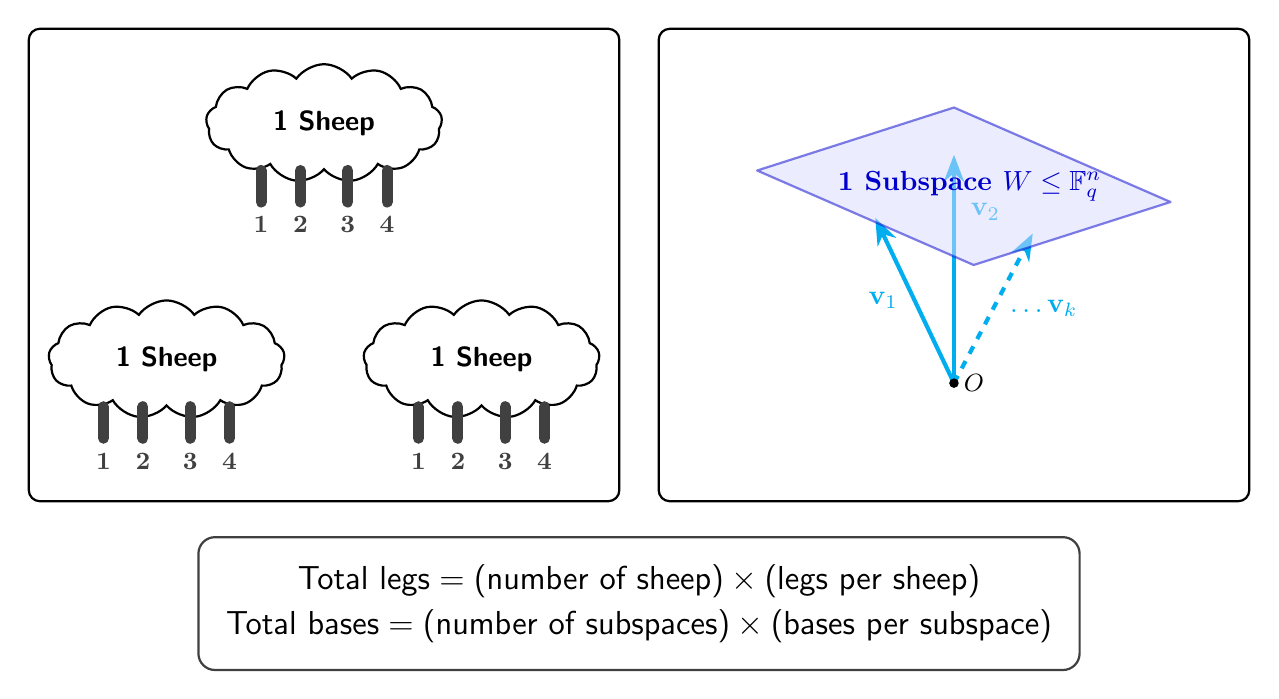
\begin{tikzpicture}[font=\sffamily]
	% --- LEFT PANEL: THE METAPHOR (SHEEP & LEGS) ---
	\node[draw, thick, rounded corners, minimum width=7.5cm, minimum height=6cm] (MetaphorBox) at (-4,0) {};
	%		\node[font=\Large\bfseries, text=green!60!black] at (-4, 2.8) {The Metaphor};
	
	\begin{scope}[shift={(0,1)}]
	% Sheep Body (The 'Space')
	\node[cloud, cloud puffs=13, cloud puff arc=110, aspect=2.2, draw=black, thick, fill=white, minimum width=3cm, minimum height=1.5cm] (Sheep) at (-4, 0.8) {\textbf{1 Sheep}};
	
	% Sheep Legs (The 'Bases')
	\draw[line width=4pt, color=darkgray, line cap=round] (-4.8, 0.2) -- (-4.8, -.2) node[below, font=\small\bfseries] {1};
	\draw[line width=4pt, color=darkgray, line cap=round] (-4.3, 0.2) -- (-4.3, -.2) node[below, font=\small\bfseries] {2};
	\draw[line width=4pt, color=darkgray, line cap=round] (-3.7, 0.2) -- (-3.7, -.2) node[below, font=\small\bfseries] {3};
	\draw[line width=4pt, color=darkgray, line cap=round] (-3.2, 0.2) -- (-3.2, -.2) node[below, font=\small\bfseries] {4};
	\end{scope}

	\begin{scope}[shift={(-2,-2)}]
		\node[cloud, cloud puffs=13, cloud puff arc=110, aspect=2.2, draw=black, thick, fill=white, minimum width=3cm, minimum height=1.5cm] (Sheep) at (-4, 0.8) {\textbf{1 Sheep}};
		
		% Sheep Legs (The 'Bases')
		\draw[line width=4pt, color=darkgray, line cap=round] (-4.8, 0.2) -- (-4.8, -.2) node[below, font=\small\bfseries] {1};
		\draw[line width=4pt, color=darkgray, line cap=round] (-4.3, 0.2) -- (-4.3, -.2) node[below, font=\small\bfseries] {2};
		\draw[line width=4pt, color=darkgray, line cap=round] (-3.7, 0.2) -- (-3.7, -.2) node[below, font=\small\bfseries] {3};
		\draw[line width=4pt, color=darkgray, line cap=round] (-3.2, 0.2) -- (-3.2, -.2) node[below, font=\small\bfseries] {4};
	\end{scope}


	\begin{scope}[shift={(2,-2)}]
		\node[cloud, cloud puffs=13, cloud puff arc=110, aspect=2.2, draw=black, thick, fill=white, minimum width=3cm, minimum height=1.5cm] (Sheep) at (-4, 0.8) {\textbf{1 Sheep}};
		
		% Sheep Legs (The 'Bases')
		\draw[line width=4pt, color=darkgray, line cap=round] (-4.8, 0.2) -- (-4.8, -.2) node[below, font=\small\bfseries] {1};
		\draw[line width=4pt, color=darkgray, line cap=round] (-4.3, 0.2) -- (-4.3, -.2) node[below, font=\small\bfseries] {2};
		\draw[line width=4pt, color=darkgray, line cap=round] (-3.7, 0.2) -- (-3.7, -.2) node[below, font=\small\bfseries] {3};
		\draw[line width=4pt, color=darkgray, line cap=round] (-3.2, 0.2) -- (-3.2, -.2) node[below, font=\small\bfseries] {4};
	\end{scope}
	
	% --- RIGHT PANEL: THE MATH (SUBSPACE & BASES) ---
	\node[draw, thick, rounded corners, minimum width=7.5cm, minimum height=6cm] (MathBox) at (4,0) {};
	%		\node[font=\Large\bfseries, text=blue!60!black] at (4, 2.8) {The Mathematics};
	
	% Origin
	\coordinate (Origin) at (4, -1.5);
	
	% Basis Vectors (The 'Legs')
	\draw[->, >=Stealth, line width=1.5pt, color=cyan] (Origin) -- (3.0, 0.6) node[midway, left=2pt] {$\mathbf{v}_1$};
	\draw[->, >=Stealth, line width=1.5pt, color=cyan] (Origin) -- (4.0, 1.4) node[near end, right=2pt] {$\mathbf{v}_2$};
	\draw[->, >=Stealth, line width=1.5pt, color=cyan, dashed] (Origin) -- (5.0, 0.4) node[midway, right=2pt] {$\dots \mathbf{v}_k$};
	
	\filldraw[black] (Origin) circle (1.5pt) node[right, font=\small\bfseries] {$O$};
	
	% Subspace Platform (The 'Sheep')
	\draw[fill=blue!15, draw=blue!80!black, thick, line join=round, opacity=.5] (1.5, 1.2) -- (4, 2.0) -- (6.75, 0.8) -- (4.25, 0.0) -- cycle;
	\node[font=\bfseries, text=blue!80!black] at (4.2, 1.0) {1 Subspace $W\leq \mathbb F_q^n$};
	
	% Bottom Summary Equation
	\node[draw=darkgray, thick, fill=white, rounded corners=6pt, minimum width=10cm, inner sep=10pt, align=center] at (0, -4.3) {
		\large $\text{Total legs} = \text{(number of sheep)}\times\text{(legs per sheep)}$\\ [4pt]
		\large $\text{Total bases} = \text{(number of subspaces)}\times\text{(bases per subspace)}$
%		\large $\displaystyle \frac{\text{Total Legs}}{\text{Legs per Sheep}} \quad \equiv \quad \frac{\text{Total Independent } k\text{-tuples}}{\text{Bases per Subspace}}$
	};
\end{tikzpicture}}
We have two steps.
\begin{enumerate}
	\item Count all ordered \(k\)-tuples $
	(\textbf{v}_1,\dots,\textbf{v}_k)$
	of linearly independent vectors in \(V\).
	\item Divide by the number of ordered bases of one fixed \(k\)-dimensional subspace.
\end{enumerate}
Then we have \[
\#\{\text{\(k\)-dimensional subspaces of }V\}
=
\frac{\#\{\text{ordered linearly independent \(k\)-tuples in }V\}}
{\#\{\text{ordered bases of one fixed \(k\)-dimensional subspace}\}}.
\]
\end{note}

%\newpage
%\vfill

\begin{tcolorbox}[colback=white, colframe=axiomcolor,title={\textbf{}}]
\begin{theorem}
Let \(V=\F_q^n\) be a $n$-dimensional $\F_2$-vector space, where \(q\) is a prime power. For \(0\le k\le n\),
\[
\#\{W\leq \F_q^n : \dim W = k\}
=
\qbinom{n}{k}
=
\prod_{i=0}^{k-1}\frac{q^n-q^i}{q^k-q^i}
=
\frac{(q^n-1)(q^n-q)(q^n-q^2)\cdots(q^n-q^{k-1})}{(q^k-1)(q^k-q)(q^k-q^2)\cdots(q^k-q^{k-1})}.
\]
\end{theorem}
\end{tcolorbox}

%\begin{proof}
%Let
%\[
%\Omega=\{(v_1,\dots,v_k)\in (\F_q^n)^k : v_1,\dots,v_k \text{ are linearly independent}\}.
%\]
%Then
%\[
%|\Omega|=(q^n-1)(q^n-q)\cdots(q^n-q^{k-1}),
%\]
%since \(v_1\) can be any nonzero vector, and after choosing \(v_1,\dots,v_i\), the next vector \(v_{i+1}\) can be any vector outside their span, which has \(q^i\) elements.
%
%On the other hand, every element of \(\Omega\) is an ordered basis of a unique \(k\)-dimensional subspace of \(\F_q^n\), and each \(k\)-dimensional subspace has exactly
%\[
%(q^k-1)(q^k-q)\cdots(q^k-q^{k-1})
%\]
%ordered bases.
%
%Therefore
%\[
%\#\{W\le \F_q^n:\dim W=k\}
%=
%\frac{(q^n-1)(q^n-q)\cdots(q^n-q^{k-1})}
%{(q^k-1)(q^k-q)\cdots(q^k-q^{k-1})}
%=
%\prod_{i=0}^{k-1}\frac{q^n-q^i}{q^k-q^i}
%=
%\qbinom{n}{k}.
%\]	
	
%We count the set
%\[
%\Omega=\{(v_1,\dots,v_k)\in (\F_q^n)^k : v_1,\dots,v_k \text{ are linearly independent}\}
%\]
%in two ways.
%
%First, we count \(\Omega\) directly. The first vector \(v_1\) may be any nonzero vector of \(\F_q^n\), so there are \(q^n-1\) choices. Once \(v_1,\dots,v_i\) have been chosen linearly independently, their span has dimension \(i\), hence contains exactly \(q^i\) vectors. Therefore \(v_{i+1}\) may be chosen arbitrarily outside this span, giving \(q^n-q^i\) choices. Thus
%\[
%|\Omega|
%=
%(q^n-1)(q^n-q)(q^n-q^2)\cdots(q^n-q^{k-1}).
%\]
%
%Next, we count \(\Omega\) by first choosing the subspace spanned by the tuple. Every element \((v_1,\dots,v_k)\in\Omega\) is an ordered basis of the \(k\)-dimensional subspace
%\[
%W=\langle v_1,\dots,v_k\rangle.
%\]
%Conversely, every ordered basis of a \(k\)-dimensional subspace gives an element of \(\Omega\).
%
%Now fix a \(k\)-dimensional subspace \(W\le \F_q^n\). The number of ordered bases of \(W\) is computed in exactly the same way as above, but now inside the \(k\)-dimensional space \(W\). The first basis vector may be any nonzero vector of \(W\), so there are \(q^k-1\) choices. After choosing \(i\) linearly independent vectors in \(W\), their span contains \(q^i\) vectors, so the next basis vector has \(q^k-q^i\) choices. Hence the number of ordered bases of \(W\) is
%\[
%(q^k-1)(q^k-q)(q^k-q^2)\cdots(q^k-q^{k-1}).
%\]
%
%Let
%\[
%N=\#\{W\le \F_q^n:\dim W=k\}.
%\]
%Since every \(k\)-dimensional subspace has the same number of ordered bases, counting \(\Omega\) by subspaces gives
%\[
%|\Omega|
%=
%N\,(q^k-1)(q^k-q)(q^k-q^2)\cdots(q^k-q^{k-1}).
%\]
%
%Comparing this with the first count of \(|\Omega|\), we obtain
%\[
%(q^n-1)(q^n-q)(q^n-q^2)\cdots(q^n-q^{k-1})
%=
%N\,(q^k-1)(q^k-q)(q^k-q^2)\cdots(q^k-q^{k-1}).
%\]
%Therefore
%\[
%N
%=
%\frac{(q^n-1)(q^n-q)(q^n-q^2)\cdots(q^n-q^{k-1})}
%{(q^k-1)(q^k-q)(q^k-q^2)\cdots(q^k-q^{k-1})}.
%\]
%
%Finally, this may be written as
%\[
%N
%=
%\prod_{i=0}^{k-1}\frac{q^n-q^i}{q^k-q^i}.
%\]
%By definition, this is the Gaussian binomial coefficient \(\qbinom{n}{k}\). Hence
%\[
%\#\{W\leq \F_q^n:\dim W=k\}
%=
%\qbinom{n}{k}.
%\]
%\end{proof}

\begin{center}
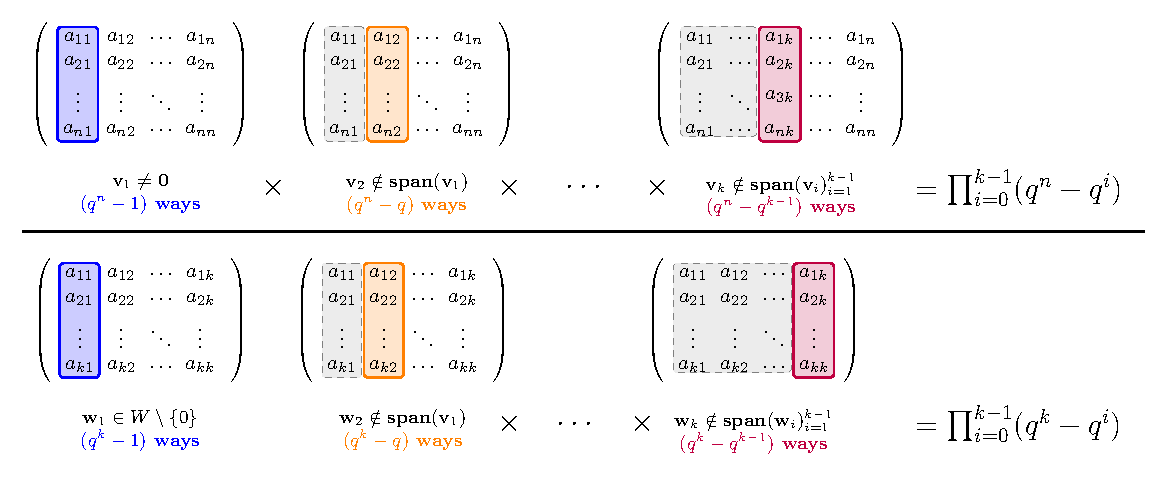
\includegraphics[width=\textwidth]{HW1/k-dim-vs-tikz1.pdf}
\end{center}

%\begin{proof}
%	We count invertible matrices by choosing their columns.
%	\begin{itemize}
%		\item The first column can be any nonzero vector of \(\F_q^m\), so there are \(q^m-1\) choices.
%		\item The second column must not lie in the span of the first column. Since the span of one nonzero vector has \(q\) elements, there are \(q^m-q\) choices.
%		\item The third column must not lie in the span of the first two columns. If those are independent, their span has \(q^2\) elements, so there are \(q^m-q^2\) choices.
%		\item Continuing this way, the \(k\)-th column must avoid a subspace of size \(q^{k-1}\), so there are \(q^m-q^{k-1}\) choices.
%	\end{itemize}
%	Multiplying all factors gives
%	\[
%	|\GL_m(\F_q)| = (q^m-1)(q^m-q)(q^m-q^2)\cdots(q^m-q^{m-1}) = \prod_{i=0}^{m-1}(q^m-q^i).
%	\]
%\end{proof}

\medskip



\newpage


%\vfill
%\footer{Department of Cyber Security\\ [4pt]
%%	College of Science and Technology\\
%	Kookmin University}
\end{document}